\hyphenation{Egerváry}
\section{Egerváry algoritmusa, az optimális hozzárendelés problémája}

Az optimális hozzárendelés problémája a következő kérdésre keresi a választ:
hogyan rendelünk egymáshoz két halmaz elemeit valamilyen optimalitási kritérium
szerint? Ilyen kritériumok lehetnek a maximális párositás, minimális idő igény
és így tovább. Grafikusan ábrázolva, legyen:

\begin{figure}[ht]
\caption{Egy optimális hozzárendelés probléma}
\label{fig:OptHozProb}
\centering 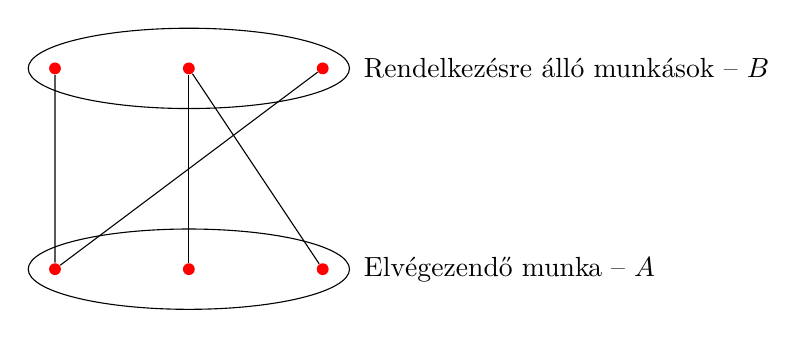
\begin{tikzpicture}[scale=1.7]
  \tikzset{ p/.style={circle,yellow,fill=red,inner sep=0pt,minimum size=0.15cm},
  }
 % the two sets
  \draw (0,0) ellipse (1.2cm and 0.3cm) node [right=2.1cm] {Elvégezendő munka -- $A$};
  \draw (0,1.5) ellipse (1.2cm and 0.3cm) node [right=2.1cm] {Rendelkezésre álló munkások --
  $B$};
  % the dots
  \node[p] (lB) at (-1, 0) {};
  \node[p] (lT) at (+1, 0) {}; 
  \node[p] (lC) at ( 0  , 0) {};
  
  \node[p] (rB) at (-1, 1.5) {}; 
  \node[p] (rT) at (+1, 1.5) {}; 
  \node[p] (rC) at ( 0, 1.5) {};
  
  % the connection between the dots
  \draw[-] (lT) -- (rC); 
  \draw[-] (lC) -- (rC); 
  \draw[-] (lB) -- (rB);
  \draw[-] (lB) -- (rT);
\end{tikzpicture} 
\end{figure}

Gráf alakban megfogalmazva, adott $G=(V, E)$ gráf, ahol $V=(A, B)$ és $E=(x,y)$,
ahol $x \in A$ és $ y \in B$. Megkülönböztetűnk $3$ fajta helyzetett:
\begin{description}
  \item[Maximális párositás problémája] Ekkor azt szeretnénk, hogy a párositások
  száma minnél nagyobb legyen.
  \item[Maximális sulyú párositás problémája] Ekkor létezzik minden párositásnak
  egy jósági tényezője, egy súlya: $w:E\rightarrow\mathbb{R}$; egy adott $M$
  párositás esetén $(M\subset E)$ keressük azt, amely maximális összeget ad:
  $\mbox{max}\left\{\sum_{e\in M}{w(e)}\right\}$.
  \item[Maximális teljes párositás problémája] Most olyan párositás halmazt
  keressünk amely a lehető legtőbb párositást létrehoz, a lehető legnagyobb
  összeggel. Azt, hogy ez nem ekvivalens a korábbi feladattal
  \aref{fig:OptMaxNemEkv} ábra szemlélteti. Ekkor a maximális sulyú párositást
  az $a_2-b_2$ adja, mig a maximális teljes párositás problémájára a helyes válasz
  az $a_1-b_2$ és $a_2-b_1$ élpárok. 
\end{description}

\begin{figure}[htb]
\caption{Maximális sulyú és teljes párositás probléma}
\label{fig:OptMaxNemEkv}
\centering
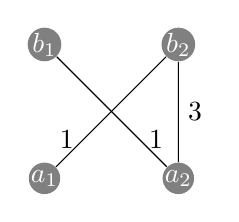
\begin{tikzpicture}[scale=1.7]
  \tikzset{
  p/.style={circle,white,fill=gray,inner sep=0pt,minimum size=0.15cm},
  }
  % the dots
  \node[p] (a1) at (0, 0) {$a_1$};
  \node[p] (a2) at (1,  0) {$a_2$};
    
  \node[p] (b1) at (0, 1) {$b_1$};
  \node[p] (b2) at (1,  1) {$b_2$};
    
  % the connection between the dots
  \draw[-] (a2) -- (b2) node [midway, right] {$3$};
  \draw[-] (a1) -- (b2) node [near start, left] {$1$};
  \draw[-] (a2) -- (b1) node [near start, right] {$1$};
\end{tikzpicture} 
\end{figure}

A maximális sulyú párositás problémája \emph{visszavezethető} a maximális sulyú
párositás problémájára. A transzformációhoz a kevesebb csucsú halmazt ($A$ és
$B$ közül) egészitsűk ki, majd a hiányzó és negativ sulyú éleken legyen $w=0$.

\subsection{Magyar módszer}

\begin{description}
  \item[Alternáló út] olyan élsorozat (séte) amely $A$-ból indul és minden második 
  él párositás beli.
  \item[Javító út] olyan alternáló út amely $B$-ben végződik.  
\end{description}

A magyar módszer lépései:
\begin{enumerate}
  \item Keresünk egy javitó útat
  \item Cseréljük meg az út menetén a szerepeket:
  	\begin{itemize}
  	\item párositásbeli élek kivétele
  	\item nem párositásbeli élek betétele 
	\end{itemize}
  \item Lépjünk vissza az első lépéshez ameddig létezik javitó út.
\end{enumerate}

\colorlet{ColorPink}{red!10}
\colorlet{ColorBlue}{blue!20}

\begin{figure}[htbp]
\caption{Magyar módszer helyessége}
\label{fig:MagyModHelyeseg}
\centering
\begin{tikzpicture}[font=\small,scale=1.7]
  \tikzset{
  p/.style={circle,white,fill=gray,inner sep=0pt,minimum size=0.15cm},
  }
  % the dots
  \draw[fill,ColorPink] (0.5,0) ellipse (0.7cm and 0.2cm) node [above=10pt,black] {$B_3$};
  \node[p] (B31) at (0,  0) {};
  \node[p] (B32) at (1,  0) {};
  
  \draw[fill,ColorBlue] (4,0) ellipse (1.5cm and 0.2cm) node [above=10pt,black] {$B_2$};
  \node[p] (B21) at (3,  0) {};
  \node[p] (B22) at (4,  0) {};
  \node[p] (B23) at (5,  0) {};
  
  \draw[fill,ColorPink] (7,0) ellipse (0.35cm and 0.2cm) node [above=10pt,black] {$B_1$};
  \node[p] (B11) at (7,  0) {};
  
  \node[p] (A31) at (0,  -1) {};
  \node[p] (A32) at (1,  -1) {};
  \draw (0.5,-1) ellipse (0.7cm and 0.2cm) node [below=10pt] {$A_3$};
  
  \draw[fill,lightgray] (4,-1) ellipse (1.5cm and 0.2cm) node [below=10pt,black] {$A_2$};
  \node[p] (A21) at (3,  -1) {};
  \node[p] (A22) at (4,  -1) {};
  \node[p] (A23) at (5,  -1) {};
  
  \draw[fill,lightgray] (7.5,-1) ellipse (0.7cm and 0.2cm) node [below=10pt,black] {$A_1$};
  \node[p] (A11) at (7,  -1) {};
  \node[p] (A12) at (8,  -1) {};
    
  \draw[-, color=blue, style=dashed] (A32) -- (B11);
  \draw[-, color=black, thick] (A31) -- (B31);
  \draw[-, color=black, thick] (A32) -- (B32);
  
  \draw[-, color=black, thick] (A21) -- (B21);
  \draw[-, color=black, thick] (A22) -- (B22);
  \draw[-, color=black, thick] (A23) -- (B23);
  
  \draw[-, color=green, thick] (A31) -- (B21);
  \draw[-, color=green, thick] (A32) -- (B31);
  \draw[-, color=green, thick] (A22) -- (B21);
  \draw[-, color=green, thick] (A22) -- (B23);
  
  \draw[-, color=green, thick] (B22) -- (A11);
  \draw[-, color=green, thick] (B23) -- (A12);
  
\end{tikzpicture} 
\end{figure} 

Az algoritmus helyeségének belátásához vegyük \aref{fig:MagyModHelyeseg} ábrát,
amely egy köztes állapotot szemléltett. Legyen:
\begin{description}
  \item[$(B_2)$] -- $A_1$--ből alternáló útón elérhető csucsok halmaza,
  \item[$(A_2)$] -- $B_2$--hőz tartozó párositás, \item[$(A_1)$] -- azon csucsók
  halamaza amelyet az $M$ párositás le nem fedett.
\end{description}

Amenyiben az algoritmus leállt $B_2$ halmaz csúcsainak végpontja $A_2$ és $A_1$
halmazból induló éleknek, azaz $B_2$ lefogó pontja az $A_1 \cup A_1$ halmaznak.
Azaz elmondható, hogy $A_3$ és $B_2$ lefogópontja a gráfnak, ugyanakkor $A_3$ és
$B_2$ elemszáma megegyezik a párositás számával. A \emph{König tétel} \footnote{
A tétel Kőnig Dénestől származik. Legyen egy $G$ páros gráf, ekkor
$\nu(G)=\tau(G)$ (azaz a legnagyobb független élhalmaznak ugyanannyi eleme van,
mint a legkisebb lefogó ponthalmaznak) és ha $G$--ben nincs izolált pont akkor
$\rho(G)=\alpha(G)$ (azaz a legkisebb lefogó élhalmaz azonos méretű a legnagyobb
független ponthalmazzal).} értelmében ezért a párositás maximális.

\subsection{Egerváry algoritmusa}

Elöszőr defináljuk a címkézés műveletet: minden csucshóz rendelünk egy valós
értéket ($c:V \rightarrow \mathbb{R}$) úgy, hogy minden élpár esetén ($\forall
\left\{x,y\right\} \in E | x \in A, y \in B$)  igaz a következő kifejezés:
$c(x)+c(y)>=w(e).$ Amenyibben $c(x)+c(y)=w(e)$ legyen az él piros. Ekkor a
maximális összsulyú teljes párositás összsúlya kisebb mint a cimkézés ősszege.

Bizonyitás:

\begin{displaymath}
\sum_M{w} \leq \sum_M{\left[c(x)+c(y)\right]} = \sum_V{c(v)}
\end{displaymath}

\emph{Lemma}: Ha $M$--ben $\forall$ él piros, a párositás maximális.

\subsection{Az algoritmus}
\begin{enumerate}
  \setcounter{enumi}{-1}
  \item lépés:  \begin{displaymath}
  c(v)=\begin{cases}
  \mbox{max}(w) & v \in A, \\
  0             & v \in B.
  \end{cases} 
  \end{displaymath}
  \item lépés: keressük meg a maximális elemszámú párositást a piros részgráfban
  javitó utakkal.
  Legyen ez a párositás $M'$. Ha ez maximális megállunk.
  \item lépesben legyen:
  \begin{displaymath}
  \begin{rcases}
  x \in A_1 \cup A_2, \\
  y \in B_1 \cup B_3\\
  \{x,y\} \in E
  \end{rcases}
  \Rightarrow \sigma= min\left\{c(x) + c(y) + w(\left\{x,y\right\}) \right\},
  \end{displaymath}
  Majd: \begin{displaymath}
  c'(v)=\begin{cases}
  c(v)-\sigma & v \in A_1 \cup A_2, \\
  c(v)+\sigma & v \in B_2, \\
  c(v) 		   &  \mbox{másképp.}
  \end{cases} 
  \end{displaymath}
  Végül legyen $M=M'$ és $c=c'$ és folytassuk az első lépéstől.
\end{enumerate} 

Az algoritmus helyeségének belátásához be kell látnunk, hogy:

\begin{enumerate}
  \item A nulladik lépés cimkézés.
  \item Létezik $\left\{x,y\right\}$ a második lépésben. Ez igaz, mert ha nem
  lenne akkor $A_1 \cup A_2$ bármely szomszédja $B_2$--ben volna és a
  \emph{Hall--feltétel} \footnote{$ \forall~x_0 \subseteq A$--ra az $|N(x_0)|
  \geq |x_0|$ egyenlőtlenségnek teljesülnie kell, másképp nem létezik párositás
  ($N~x_0$ szomszédainak halmazát fedi).} alapján nem létezne párositás.
  \item $c'$ cimkézés e? Ehhez figyeljük meg, hogy $\sigma$ hogyan változhat:
  
  \begin{tabular}{ l |  c c }
                  & $A_1 \cup A_2$ & $A_3$ \\
                  \hline
  $B_2$           & $0$            & $+\sigma$ \\
  $B_1 \cup B_3$ & $-\sigma$      & $0$ \\
  \end{tabular}
  
  Tehát a cimkézés csak egy helyt csökken (ami elronthatná a cimkézést), de itt
  csak a maximális csőkkenthető értékkel csökken, tehát a cimkézés tulajdonsága 
  megmarad.
  \item Ahol $\sigma$ minimális ott egy piros él keletkezik. Ez igaz hisszen ahol ez
  igaz ott vagy megnő $M$ élszáma (ekkor $\in B$) vagy megszűnik a piros él
  ($\in A_3 \ cup B_2$), de helyete egy új keletekezik.
  \item $B_3$ legfeljebb n lépésből elfogy. A következő lépsben $B_1$--beli a
  piros él, tehát nő a párositás $\Rightarrow n^2$ iterációba legfeljebb
  megvagyunk.
  \end{enumerate}